\section{Overall Task}
We are asked to determine if a patient is diseased or healthy from a given data set. A new test is in development and measures the concentration of 2 chemicals in urine samples. 500 patients provide urine samples and also undergo a blood tests to classify if they are diseased or healthy. Thus, we have a 500 by 2 data set which is plotted in Figure \ref{fig:trainingData}. 

\begin{figure}[h]
	\centering
	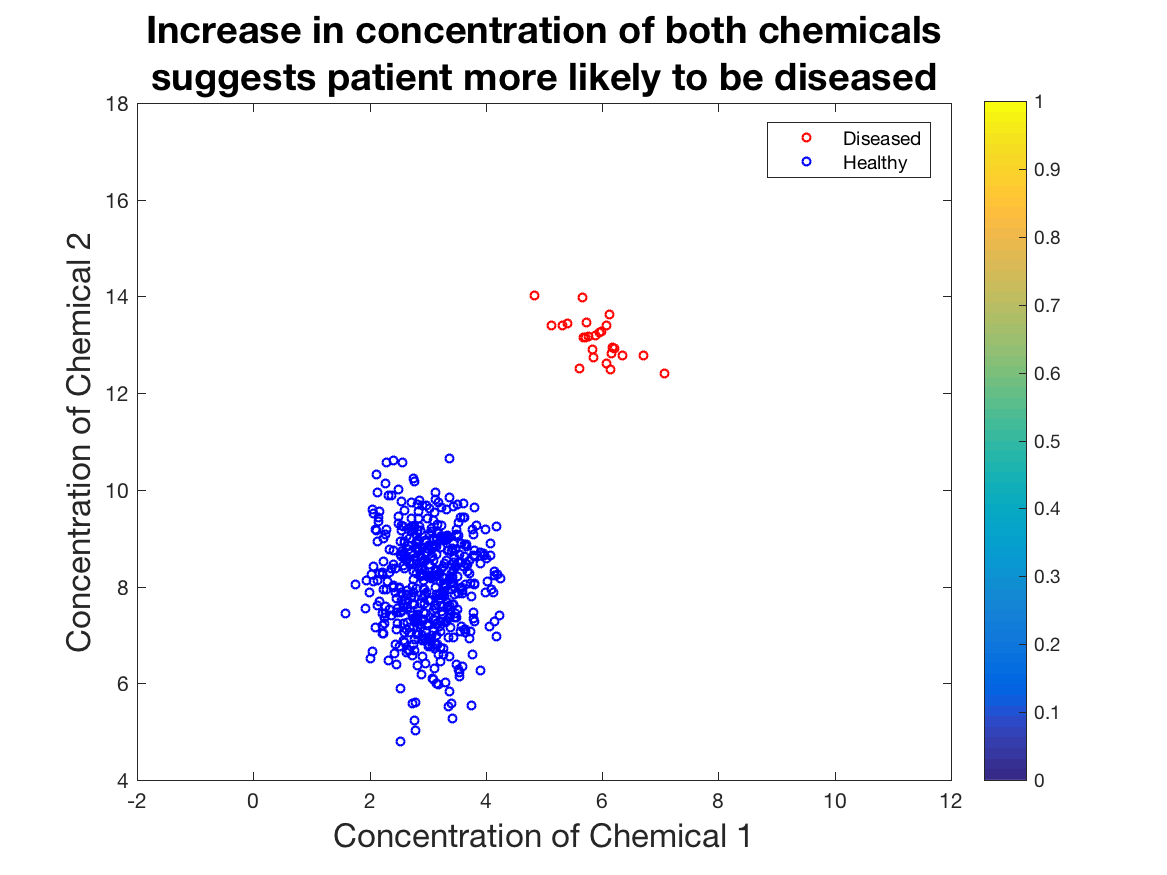
\includegraphics[width=0.8\linewidth]{images/MLtrainingData}
	\caption{Training Data for the 4 methods outlined in this report.}
	\label{fig:trainingData}
\end{figure}

We use this data set to train the 4 following methods. 

\begin{itemize}
	\item Maximum Likelihood (ML) - Appendix A
	\item Maximum Likelihood without Naive assumption (MLWON) - Appendix B
	\item Maximum a posteriori (MAP) - Appendix C
	\item Maximum a posteriori without Naive assumption(MAPWON) - Appendix D
\end{itemize}

The analysis was done in Matlab and the code listings for each method are found in the Appendices as described above. Appendix E contains a code listing for a program comparing the classification of each method.

Note the code is separated into `Analysis' and `Plots.' The `Analysis' part is the algorithm for each respective classification method. The `Plots' part can be disregarded unless the reader is interested in how the plots were generated.

Once trained, we are tasked with classifying 2000 new urine samples. We use the 4 methods outlined previously to determine whether a `patient' is diseased or healthy. 

It is helpful to state a hypothesis for assessment. Considering the data in Figure \ref{fig:trainingData} the hypothesis is, an increase in concentration of chemical 1 and 2 increases the likelihood of a patient being diagnosed as diseased.

\section{Task 1 - Maximum Likelihood}
In Task 1, we are asked to ``train the Bayesian classifier, with maximum likelihood estimate (ML), on the training data (Figure \ref{fig:trainingData}) with and without the Naive assumption.'' Once trained, we classify 2000 new data points (patients).

To train ML with the Naive assumption we first compute the mean and variance of the data for each class and attribute. As it is Naive, we assume the attributes (chemical 1 and 2) are independent. Armed with the mean, variance, and the new data set, we use the Gaussian expression to compute the likelihood of each data point being diseased or healthy. In this case, we are looking at the Maximum Likelihood and thus, only use class-conditional likelihood to classify. Refer Figure \ref{fig:ML} for classification without the Naive assumption.

\begin{figure}[h]
	\centering
	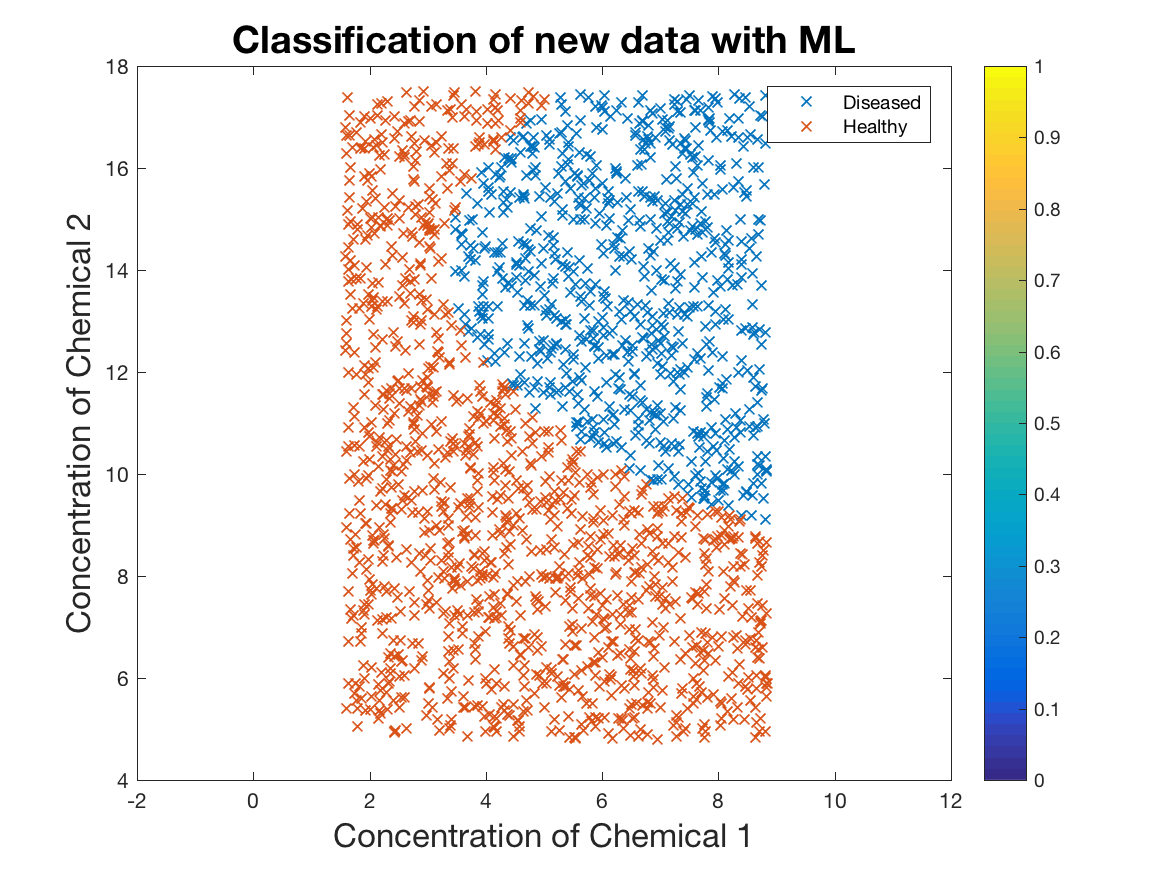
\includegraphics[width=0.8\linewidth]{images/MLnewData}
	\caption{Maximum Likelihood classification of new data}
	\label{fig:ML}
\end{figure}

Training ML without the Naive assumption is similar to before. We compute the mean as normal but this method requires the covariance, not variance, of the attributes for each class. This allows us to model any dependence between the attributes. We then compute the maximum likelihood as normal but accounting for the 3 dimensional matrix due to the covariance of each class. Refer Figure \ref{fig:MLWON} for classification with the Naive assumption.

\begin{figure}[h]
	\centering
	\includegraphics[width=0.8\linewidth]{images/MLWONnewData}
	\caption{Maximum Likelihood without Naive assumption classification of new data}
	\label{fig:MLWON}
\end{figure}

Refer Figure \ref{fig:CMLdens} for plots of the class-conditional density contours for the 2 ML methods. These plots show the mean of the data by the centre of the contours. The spread of the data is represented by the proximity of contours lines i.e. closer contour lines equals smaller spread. Dependence between attributes is shown by tilted contours i.e. downward tilt is a negative relationship.

\begin{figure}[h!] 
	\centering
	\begin{subfigure}[b]{.40\textwidth}
		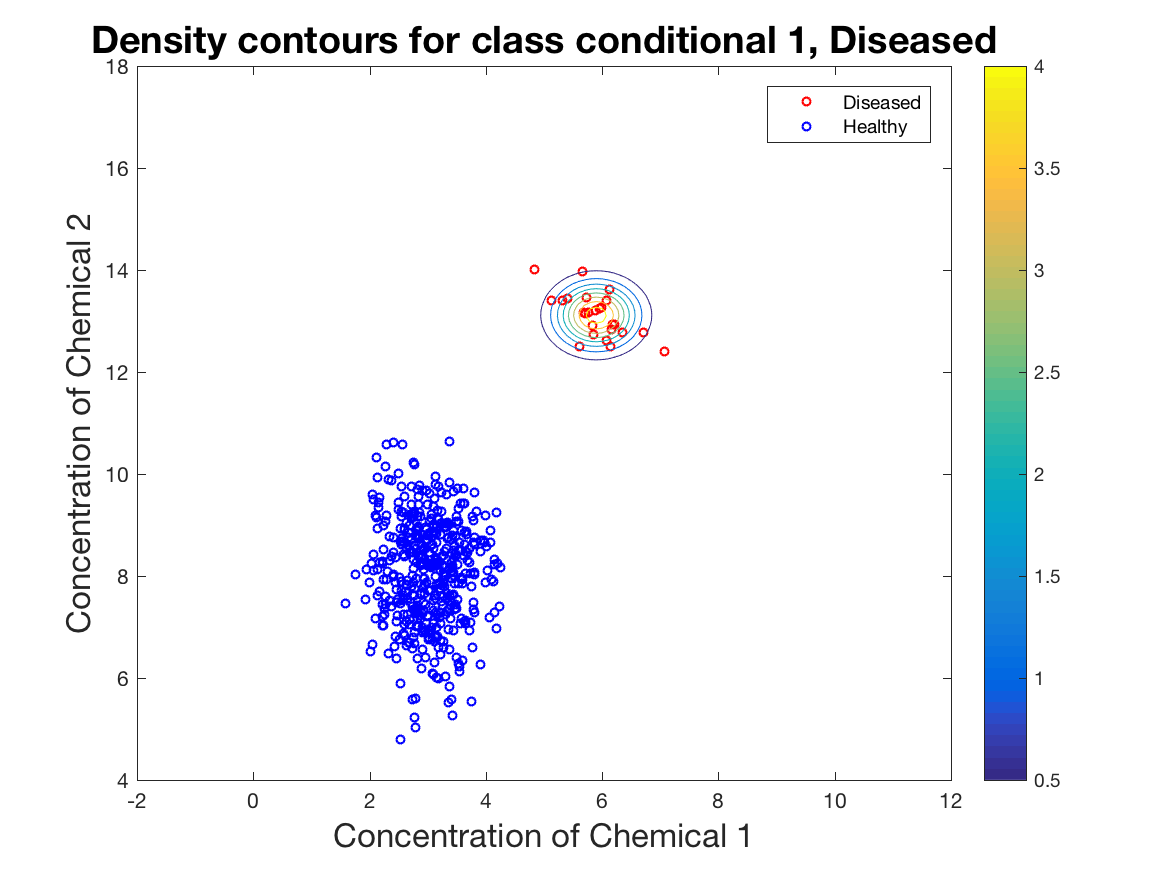
\includegraphics[width=\textwidth]{MLclassCondContoursDiseased.png}
		\caption{ML class conditional 1 density contours}
		\label{fig:cml1}
	\end{subfigure}
	\begin{subfigure}[b]{.40\textwidth}
		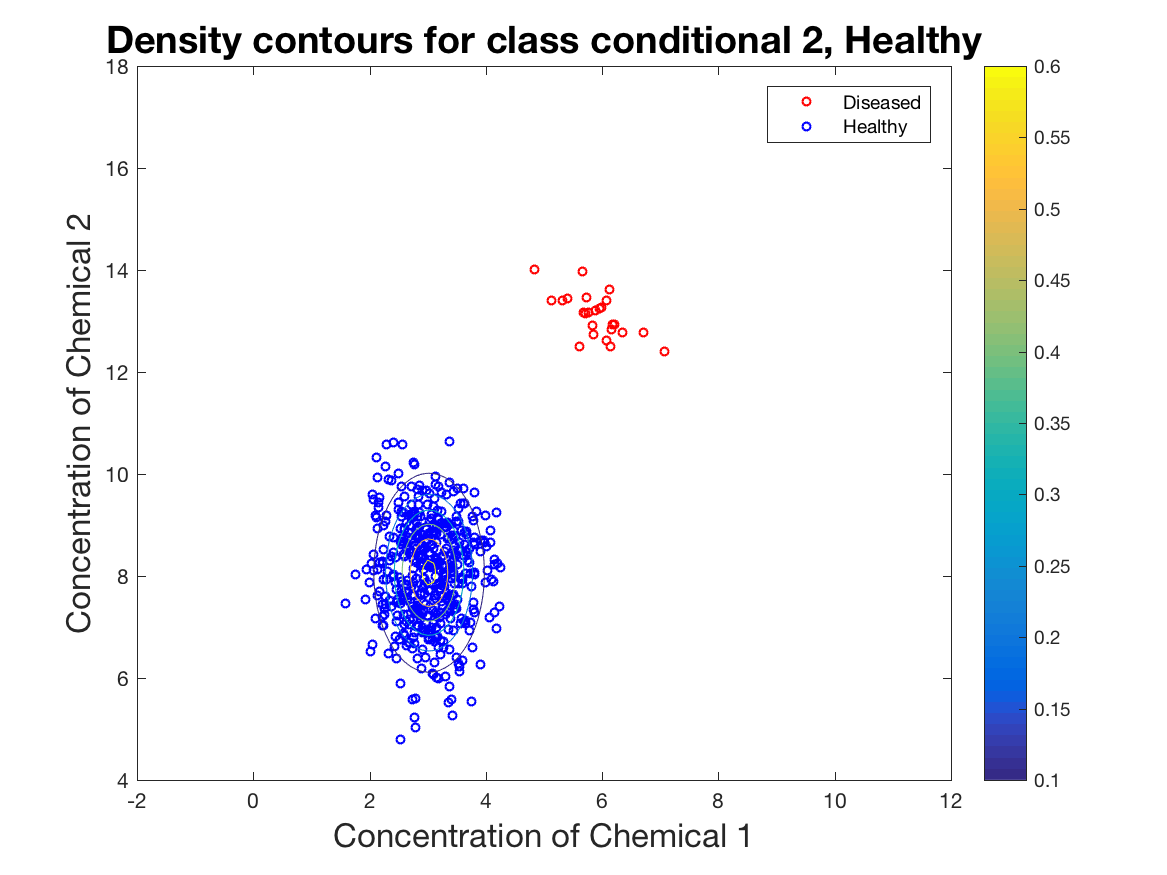
\includegraphics[width=\textwidth]{MLclassCondContoursHealthy.png}
		\caption{ML class conditional 2 density contours}
		\label{fig:cml2}
	\end{subfigure}
	\begin{subfigure}[b]{.40\textwidth}
		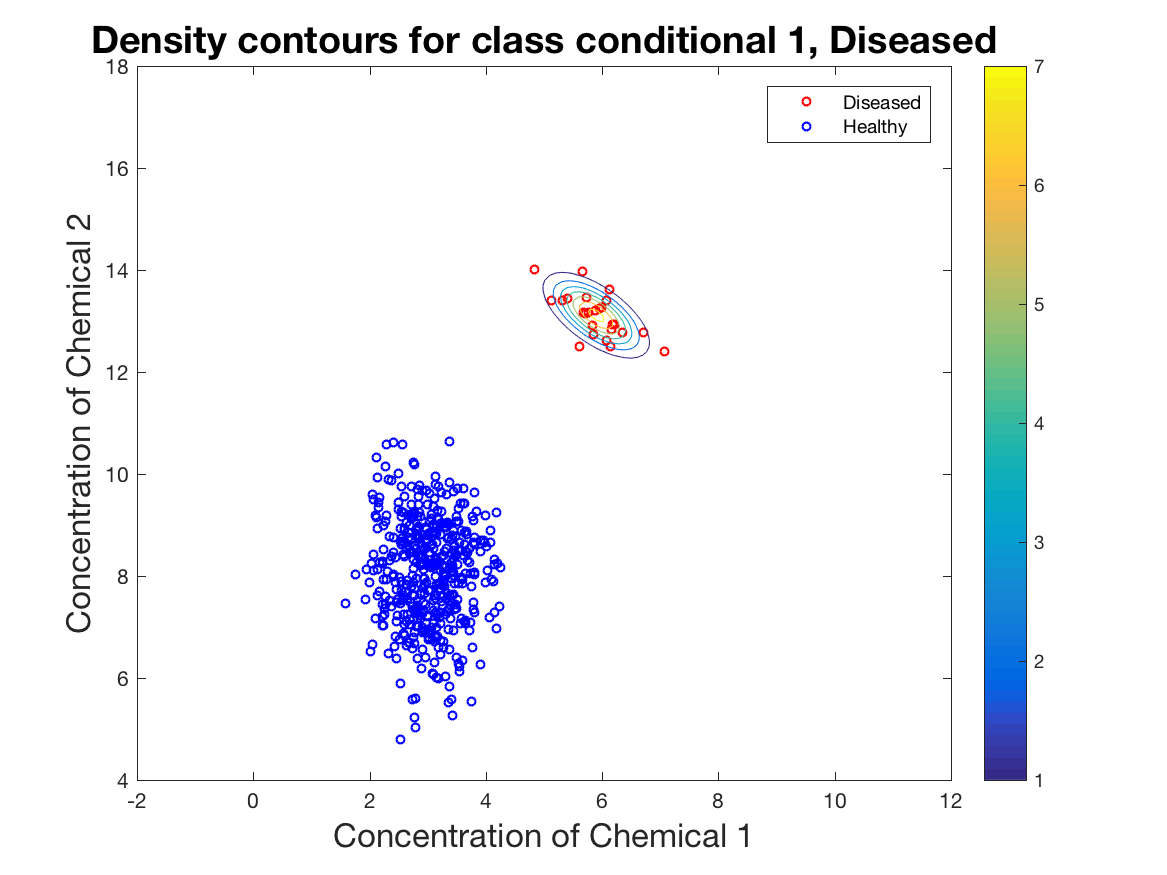
\includegraphics[width=\textwidth]{MLWONclassCondContoursDiseased.png}
		\caption{MLWON class conditional 1 density contours}
		\label{fig:cml3}
	\end{subfigure}
	\begin{subfigure}[b]{.40\textwidth}
		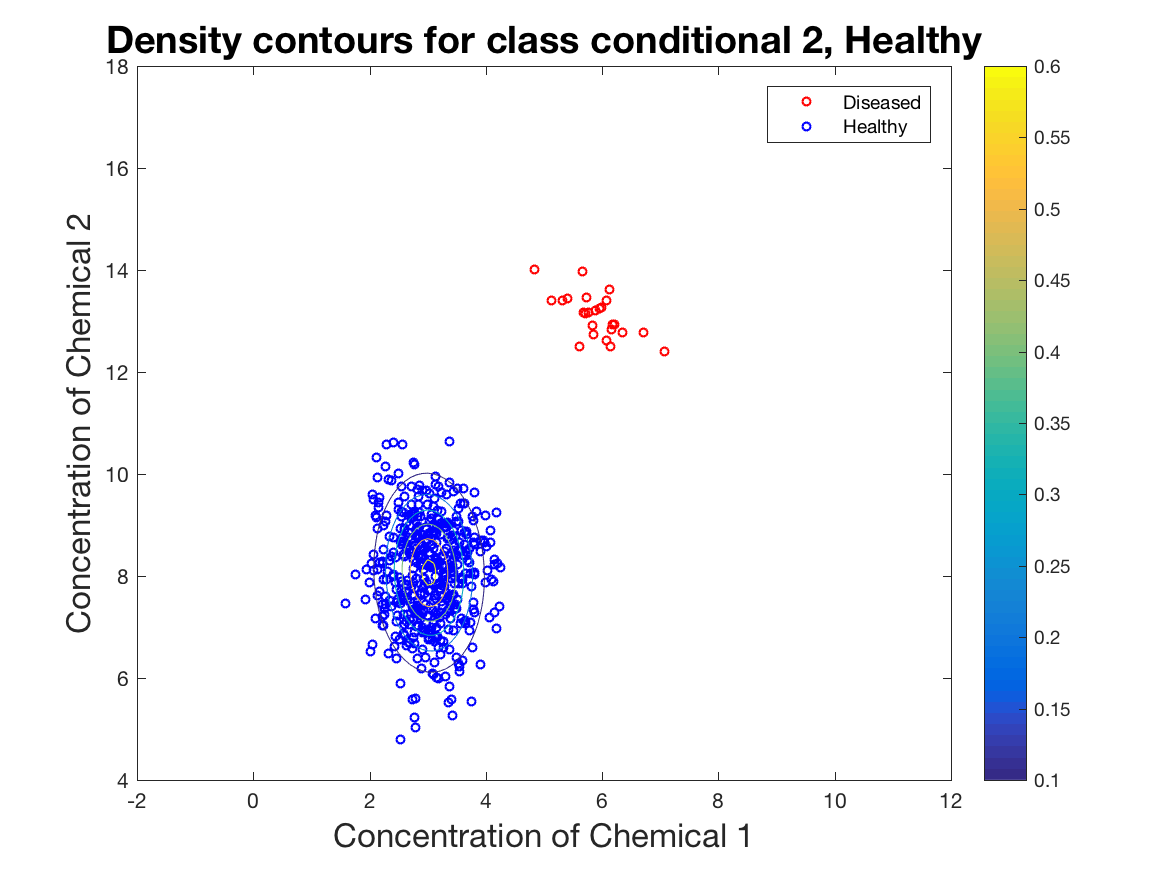
\includegraphics[width=\textwidth]{MLWONclassCondContoursHealthy.png}
		\caption{MLWON class conditional 2 density contours}
		\label{fig:cml4}
	\end{subfigure}
	\caption{Comparison of ML class conditional density contours for each class and with Naive and without Naive assumption}
	\label{fig:CMLdens}
\end{figure}

The mean of the training data is shown in Table \ref{t:mean}. The mean of the healthy patients is represented by (5.90, 13,11) and for diseased it is (3.02, 8.06).

\begin{table}[h]
	\centering
	\caption{Mean of Diseased and Healthy Class for Training Data}
	\label{t:mean}
	\begin{tabular}{lrr}
		\hline
		\textbf{Class} & \textbf{Chemical 1} & \textbf{Chemical 2} \\ \hline
		Diseased & 5.90 & 13.113 \\
		Healthy & 3.02 & 8.06  \\
	\end{tabular}
\end{table}

Tables \ref{t:var1} and \ref{t:var2}, show the covariance for the diseased and healthy patients respectively. Note, this is with the Naive assumption, therefore, the off diagonal elements are zero (independence).

\begin{table}[h!]
	\centering
	\caption{Class 1 (Diseased) variance of Chemical Concentrations for ML (or MAP)}
	\label{t:var1}
	\begin{tabular}{lrr}
		\hline
		\textbf{} & \textbf{Chemical 1} & \textbf{Chemical 2} \\ \hline
		Chemical 1 & 0.210 & 0.0 \\
		Chemical 2 & 0.0 & 0.176  \\
	\end{tabular}
\end{table}

\begin{table}[h!]
	\centering
	\caption{Class 2 (Healthy) variance of Chemical Concentrations for ML (or MAP)}
	\label{t:var2}
	\begin{tabular}{lrr}
		\hline
		\textbf{} & \textbf{Chemical 1} & \textbf{Chemical 2} \\ \hline
		Chemical 1 & 0.247 & 0.0 \\
		Chemical 2 & 0.0 & 1.045 \\
	\end{tabular}
\end{table}

Tables \ref{t:cov1} and \ref{t:cov2}, show the covariance for the diseased and healthy patients respectively. Note, this is without the Naive assumption, therefore, the off diagonal elements are not zero (dependence).

\begin{table}[h]
	\centering
	\caption{Class 1 (Diseased) Covariance of Chemical Concentrations for ML (or MAP) WON}
	\label{t:cov1}
	\begin{tabular}{lrr}
		\hline
		\textbf{} & \textbf{Chemical 1} & \textbf{Chemical 2} \\ \hline
		Chemical 1 & 0.210 & -0.124 \\
		Chemical 2 & -0.124 & 0.176  \\
	\end{tabular}
\end{table}

\begin{table}[h]
	\centering
	\caption{Class 2 (Healthy) Covariance of Chemical Concentrations for ML (or MAP) WON}
	\label{t:cov2}
	\begin{tabular}{lrr}
		\hline
		\textbf{} & \textbf{Chemical 1} & \textbf{Chemical 2} \\ \hline
		Chemical 1 & 0.247 & -0.023 \\
		Chemical 2 & -0.023 & 1.045  \\
	\end{tabular}
\end{table}

Refer to Figure \ref{fig:CMLprob} for the probability contours of the Maximum Likelihood. These plots show the likelihood of classification for any value of the 2 attributes. For example, in the top-right of Figure \ref{fig:cmlprob1}, there is high probability of diseased classification as it is within the yellow contour line (probability > 0.9).

\begin{figure}[h!] 
	\centering
	\begin{subfigure}[b]{.40\textwidth}
		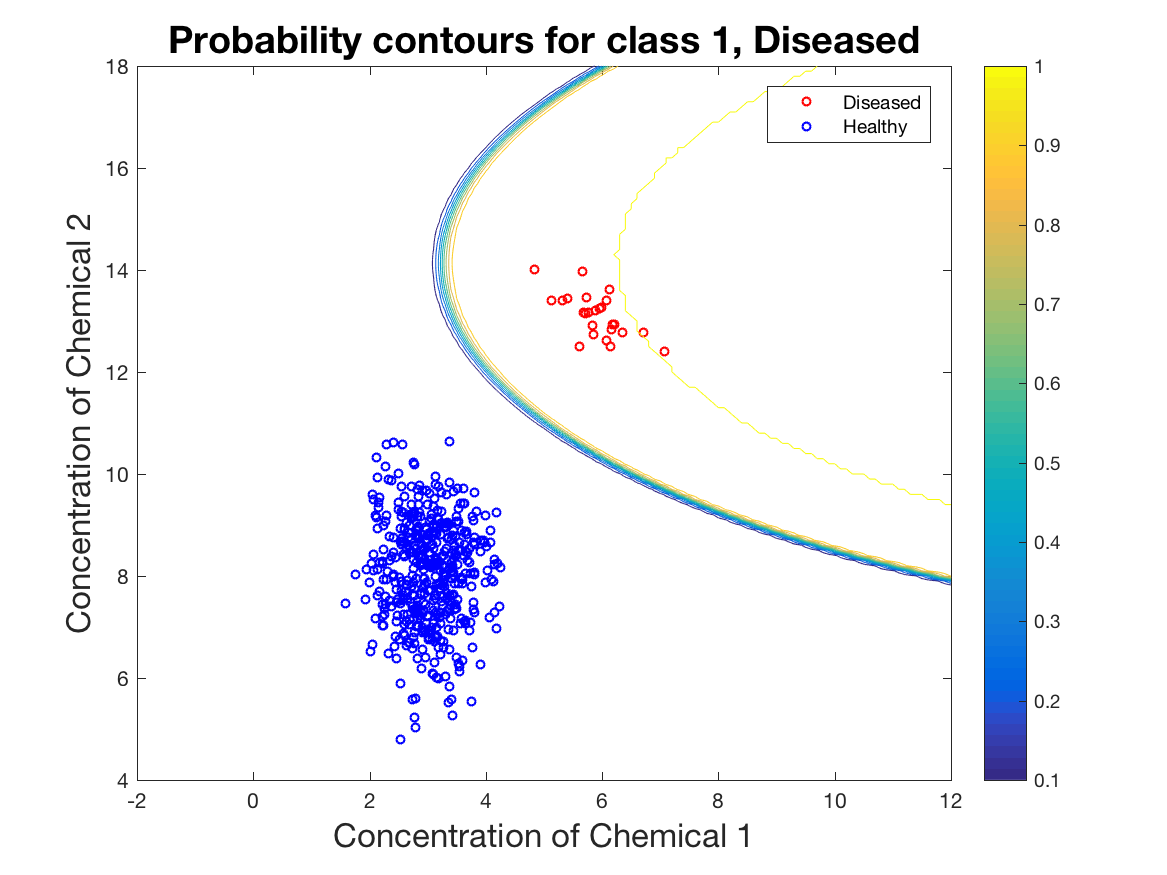
\includegraphics[width=\textwidth]{MLprobContoursDiseased.png}
		\caption{ML probability contours for class 1}
		\label{fig:cmlprob1}
	\end{subfigure}
	\begin{subfigure}[b]{0.40\textwidth}
		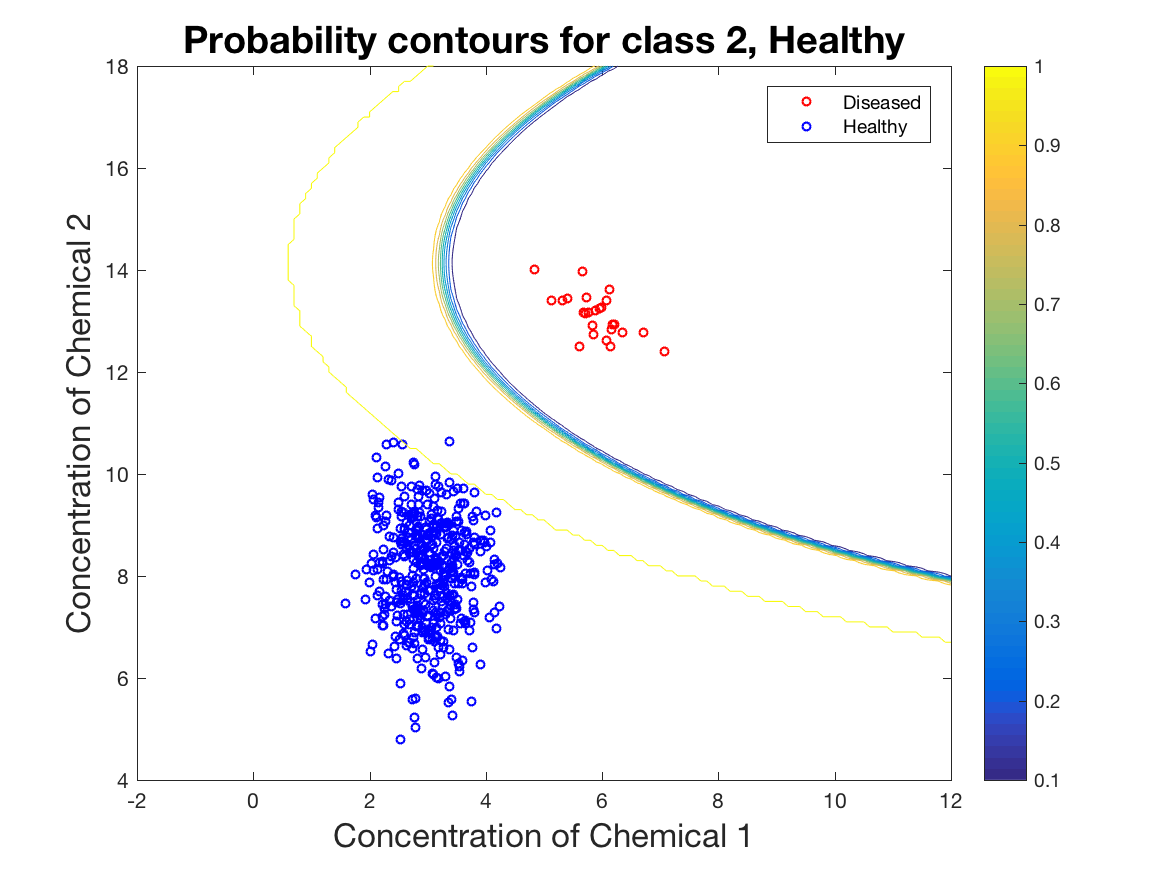
\includegraphics[width=\textwidth]{MLprobContoursHealthy.png}
		\caption{ML probability contours for class 2}
		\label{fig:model1}
	\end{subfigure}
	\begin{subfigure}[b]{.40\textwidth}
		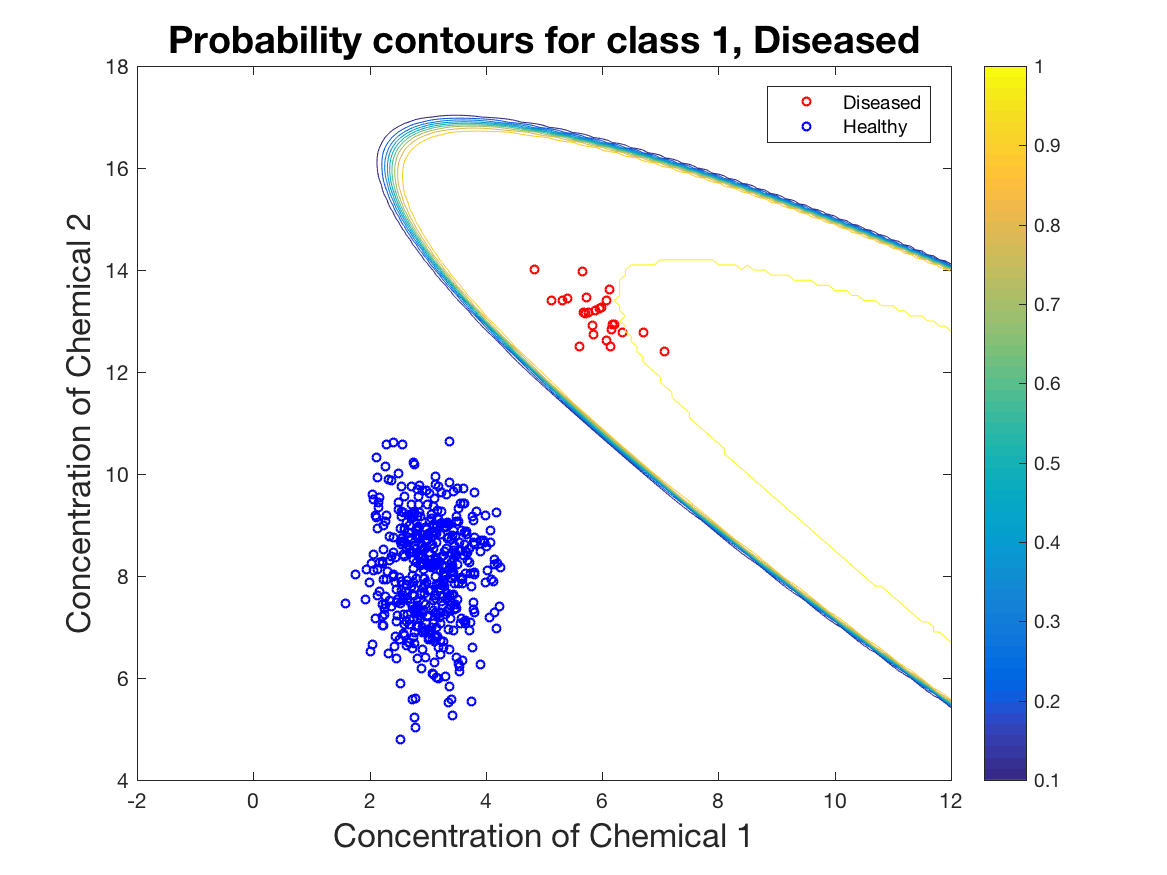
\includegraphics[width=\textwidth]{MLWONprobContoursDiseased.png}
		\caption{MLWON probability contours for class 1}
		\label{fig:model2}
	\end{subfigure}
	\begin{subfigure}[b]{.40\textwidth}
		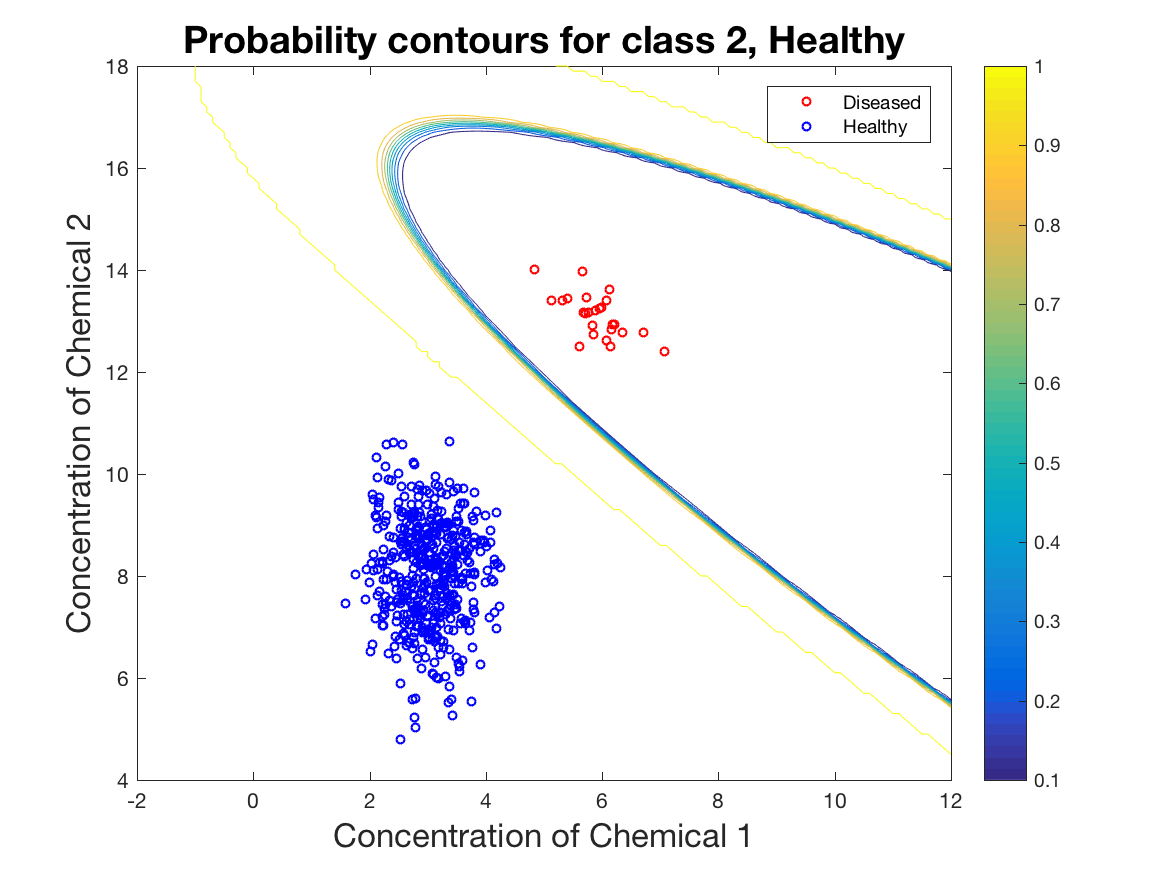
\includegraphics[width=\textwidth]{MLWONprobContoursHealthy.png}
		\caption{MLWON probability contours for class 2}
		\label{fig:model3}
	\end{subfigure}
	\caption{Comparison of ML probability contours for each class and with Naive and without Naive assumption}
	\label{fig:CMLprob}
\end{figure}


\section{Task 2- Maximum a posteriori}
In Task 2, we are asked to ``train the Bayesian classifier, with Maximum a Posteriori (ML), on the training data (Refer Figure \ref{fig:trainingData}) with and without the Naive assumption.'' Once trained, we classify 2000 new data points (patients).

To train MAP with the Naive assumption is the same as ML, except we multiply the ML by the prior. Where the prior is the probability of each class. The affects of the prior is discussed further in Section \ref{MLvMAP}. Refer Figure \ref{fig:MAP} for classification with the Naive assumption.

\begin{figure}[h]
	\centering
	\includegraphics[width=0.8\linewidth]{images/MAPnewData}
	\caption{Maximum a posteriori classification of new data}
	\label{fig:MAP}
\end{figure}

Training MAP without the Naive assumption is similar to ML without the Naive assumption except we multiply by the prior. Refer Figure \ref{fig:MAPWON} for classification without the Naive assumption.

\begin{figure}[h]
	\centering
	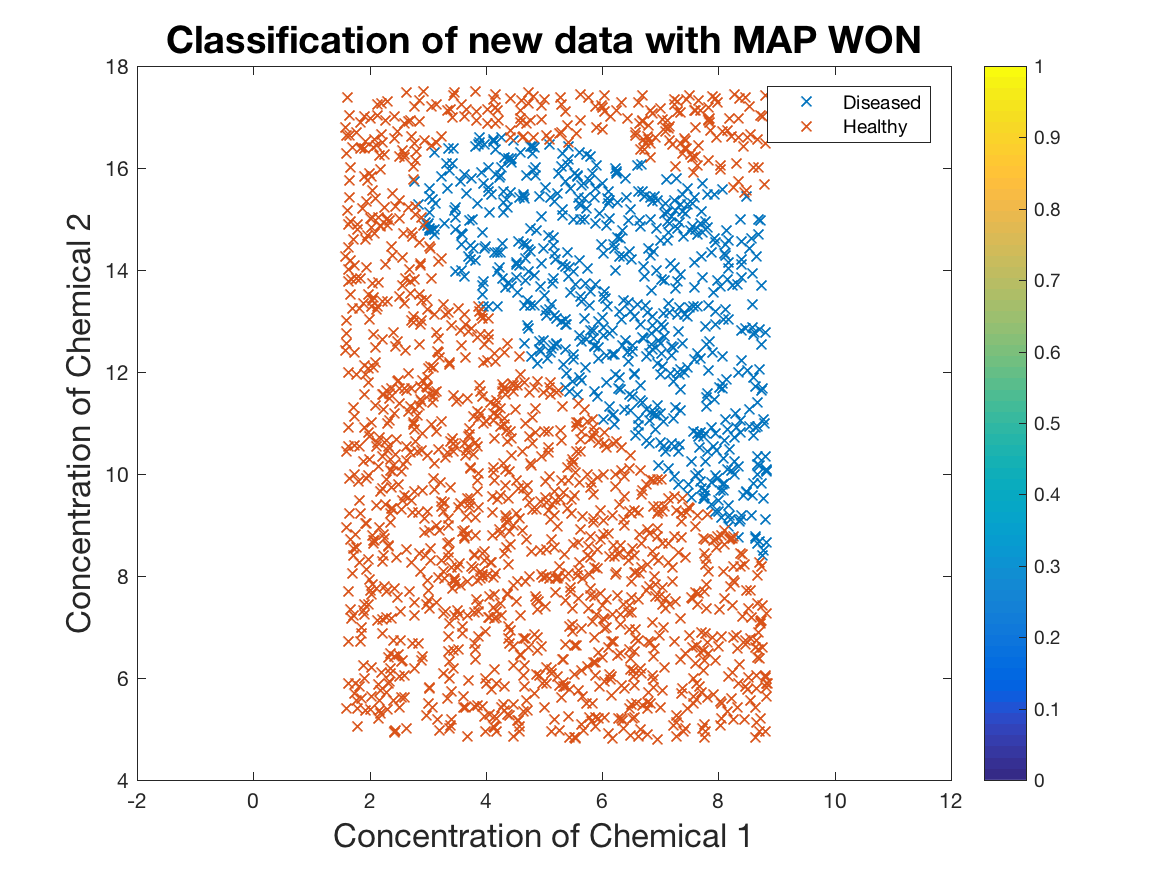
\includegraphics[width=0.8\linewidth]{images/MAPWONnewData}
	\caption{Maximum a posteriori without Naive assumption classification of new data}
	\label{fig:MAPWON}
\end{figure}

Refer Figure \ref{fig:CMAPdens} for plots of the density contours for the 2 MAP methods. These plots show the mean of the data by the centre of the contours. The spread of this data is represented by the proximity of the contours i.e close contour lines indicate small spread. Dependence between the attributes is shown by the tilted contours i.e. downward tilt is a negative relationship.

\begin{figure}[h!] 
	\centering
	\begin{subfigure}[b]{.49\textwidth}
		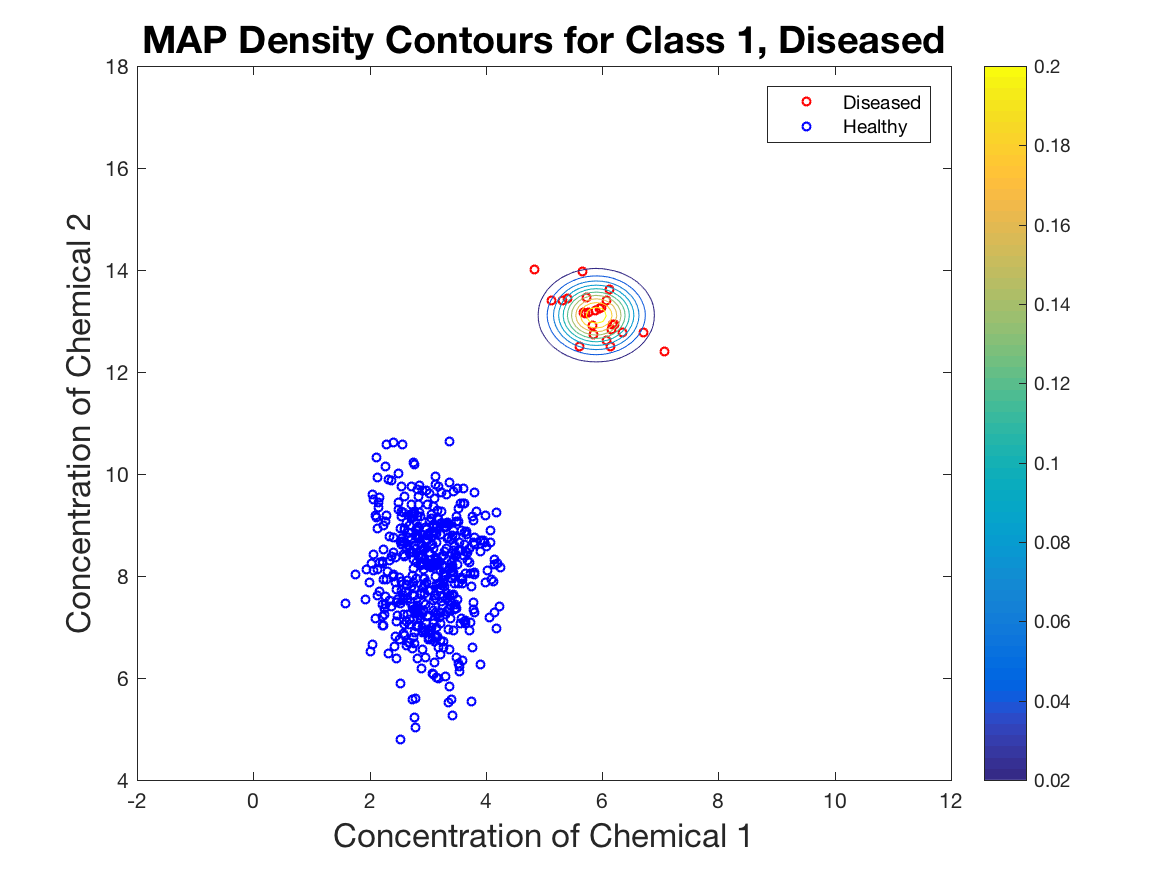
\includegraphics[width=\textwidth]{MAPclassCondContoursDiseased.png}
		\caption{MAP density contours for class 1}
		\label{fig:model0}
	\end{subfigure}
	\begin{subfigure}[b]{.49\textwidth}
		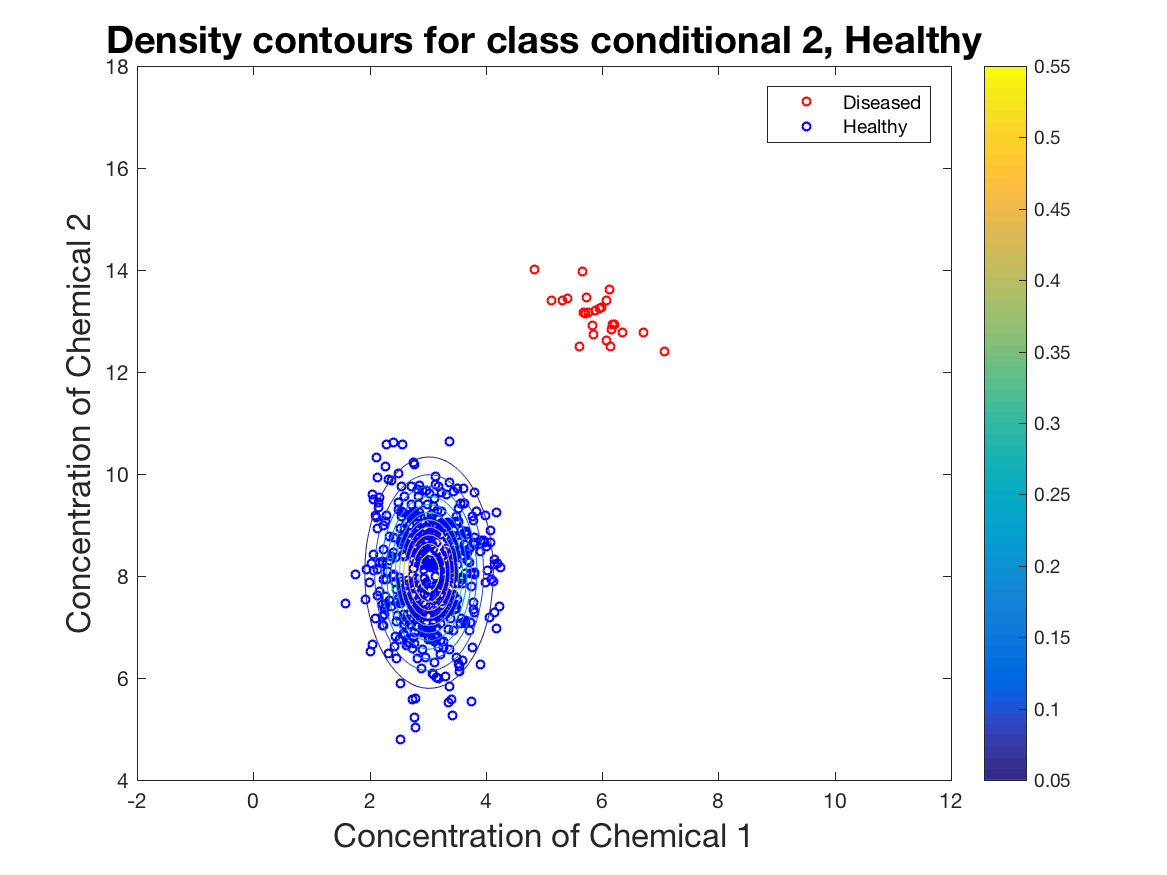
\includegraphics[width=\textwidth]{MAPclassCondContoursHealthy.png}
		\caption{MAP density contours for class 2}
		\label{fig:model1}
	\end{subfigure}
	\begin{subfigure}[b]{.49\textwidth}
		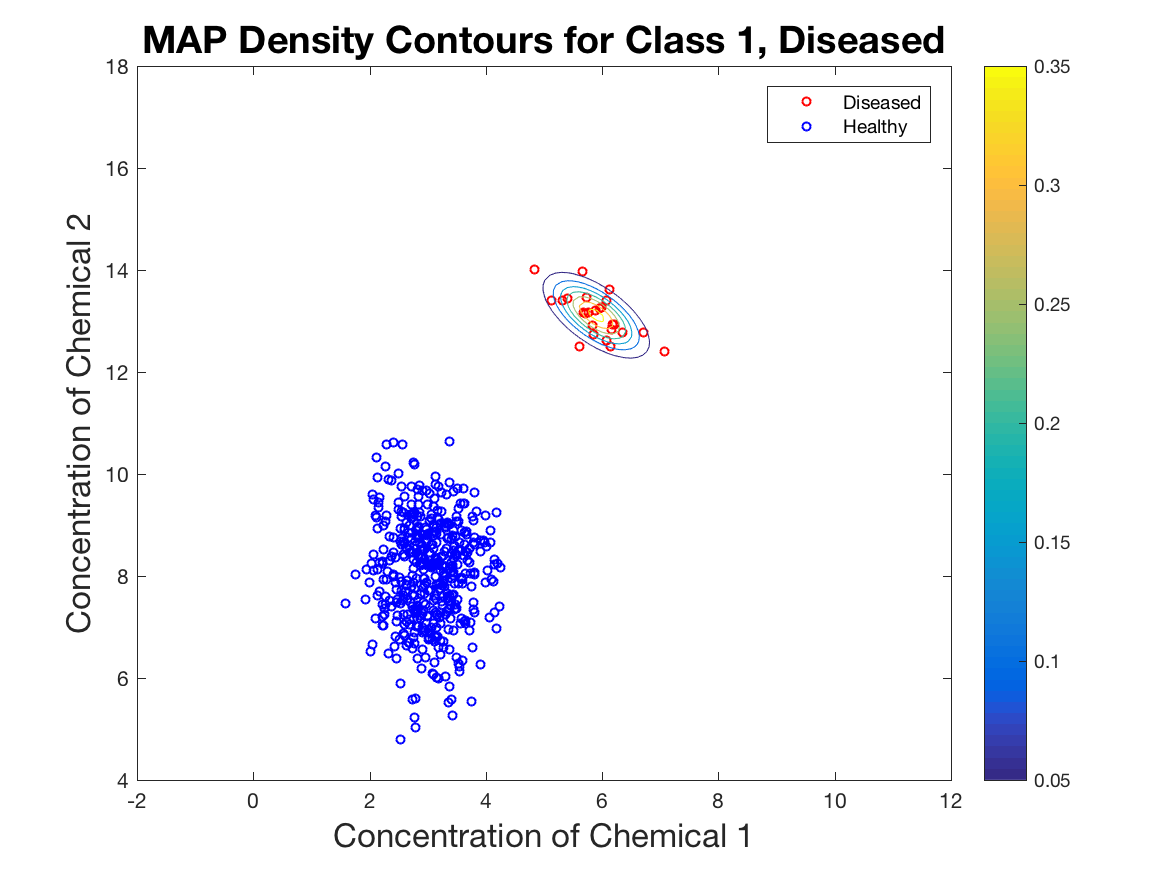
\includegraphics[width=\textwidth]{MAPWONclassCondContoursDiseased.png}
		\caption{MAPWON density contours for class 1}
		\label{fig:model2}
	\end{subfigure}
	\begin{subfigure}[b]{.49\textwidth}
		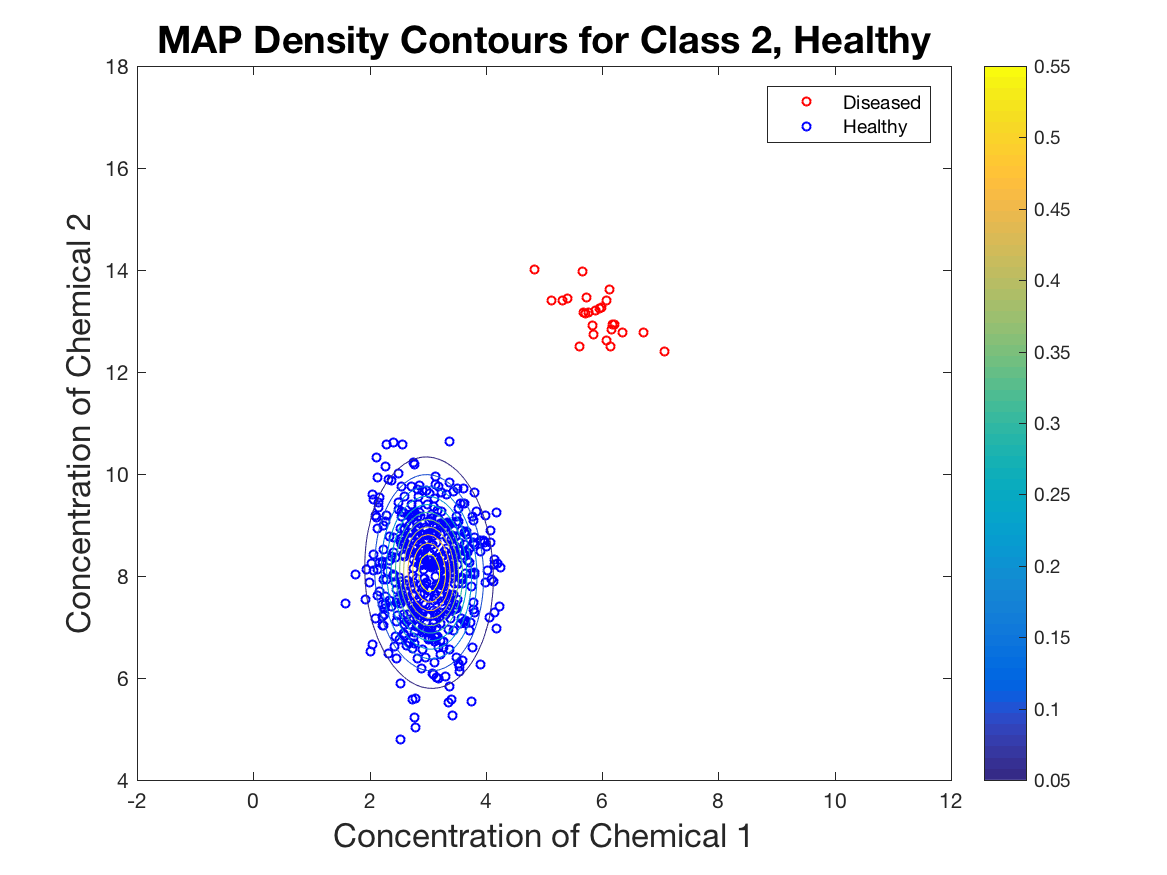
\includegraphics[width=\textwidth]{MAPWONclassCondContoursHealthy.png}
		\caption{MAPWON density contours for class 2}
		\label{fig:model3}
	\end{subfigure}
	\caption{Comparison of MAP density contours for each class and with Naive and without Naive assumption}
	\label{fig:CMAPdens}
\end{figure}

The mean is the same as before and is shown in Table \ref{t:mean}. To reiterate, the healthy patients have mean (5.90, 13,11) and diseased have (3.02, 8.06).

The covariance is the same as outlined in the Maximum Likelihood method. Refer to the previous section for the explanation of interpreting the Tables \ref{t:var1}, \ref{t:var2}, \ref{t:cov1}, and \ref{t:cov2}.

Refer to Figure \ref{fig:CMAPprob} for the probability contours of the Maximum a posteriori. These plots show the likelihood of classification for any value of the 2 attributes. For example, in the top-right of Figure \ref{fig:cmapprob1}, there is high probability of diseased classification as it is within the yellow contour line (probability > 0.9). 

\begin{figure}[h!] 
	\centering
	\begin{subfigure}[b]{.49\textwidth}
		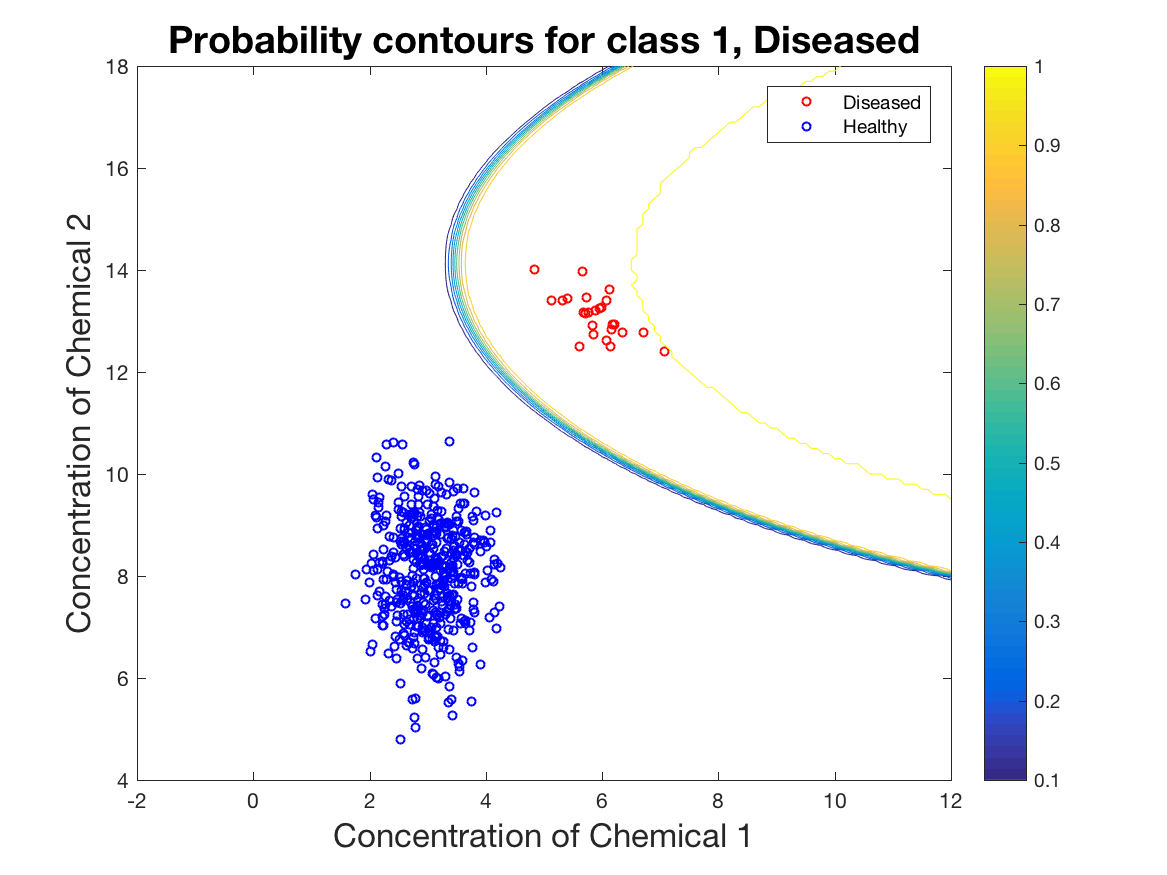
\includegraphics[width=\textwidth]{MAPprobContoursDiseased.png}
		\caption{MAP probability contours for class 1}
		\label{fig:cmapprob1}
	\end{subfigure}
	\begin{subfigure}[b]{.49\textwidth}
		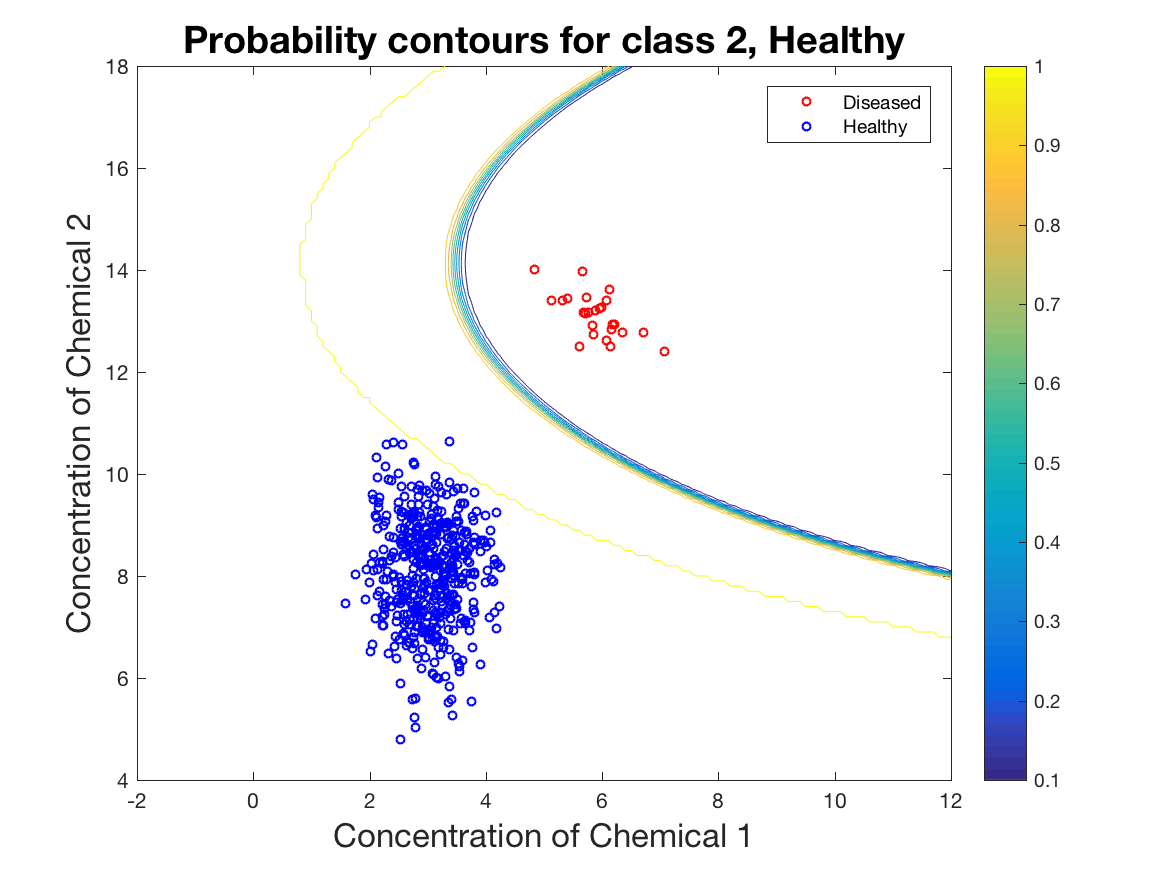
\includegraphics[width=\textwidth]{MAPprobContoursHealthy.png}
		\caption{MAP probability contours for class 2}
		\label{fig:model1}
	\end{subfigure}
	\begin{subfigure}[b]{.49\textwidth}
		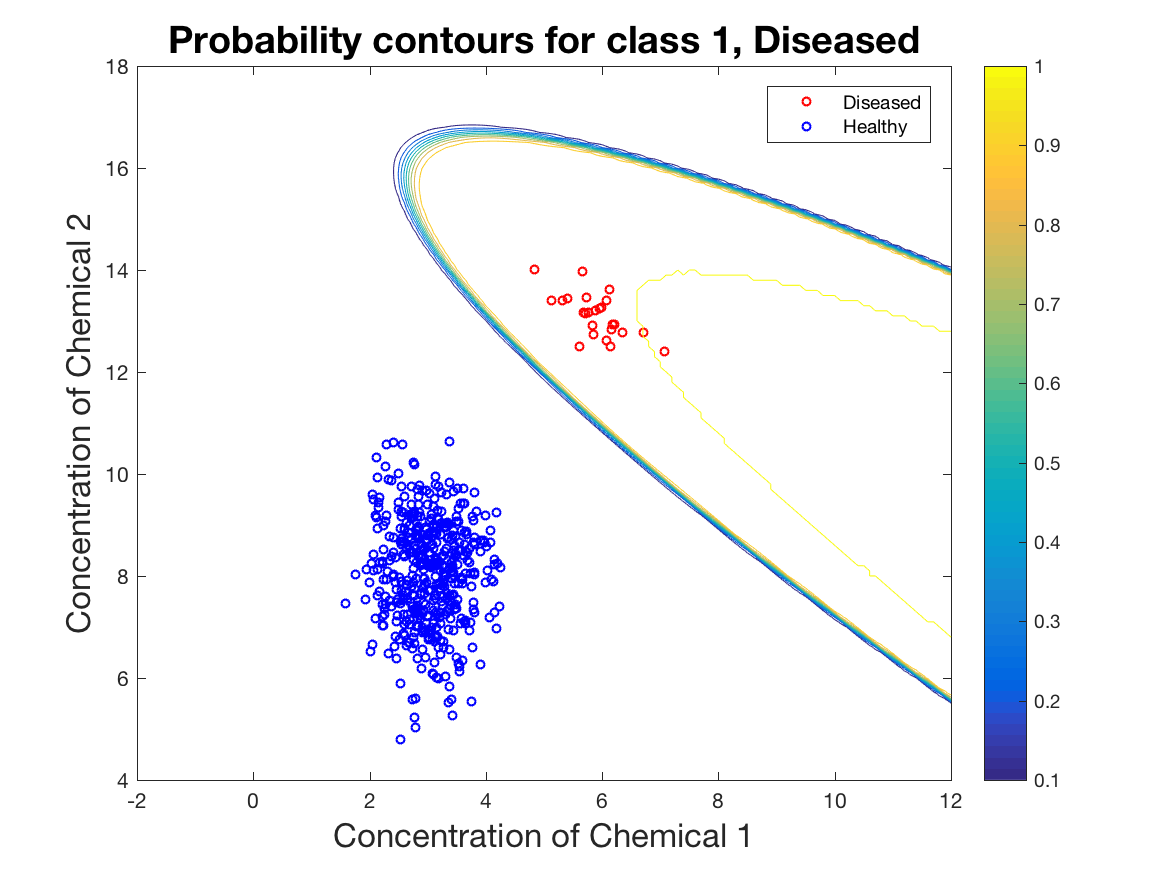
\includegraphics[width=\textwidth]{MAPWONprobContoursDiseased.png}
		\caption{MAPWON probability contours for class 1}
		\label{fig:model2}
	\end{subfigure}
	\begin{subfigure}[b]{.49\textwidth}
		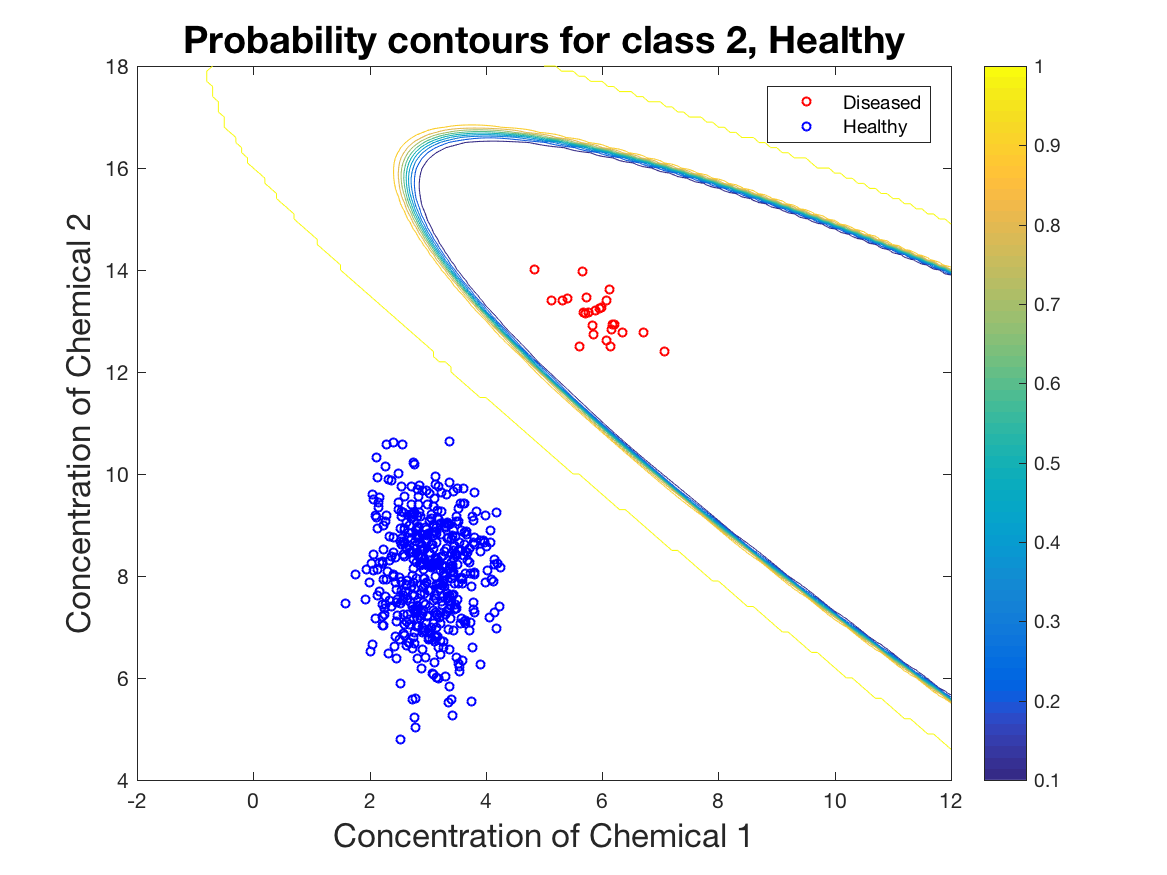
\includegraphics[width=\textwidth]{MAPWONprobContoursHealthy.png}
		\caption{MAPWON probability contours for class 2}
		\label{fig:model3}
	\end{subfigure}
	\caption{Comparison of MAP probability contours for each class and with Naive and without Naive assumption}
	\label{fig:CMAPprob}
\end{figure}

\section{Comparison of Naive vs Without Naive}{\label{s1}
	
\subsection{Introduction}\label{Int}
For simplicity we refer only to Maximum Likelihood (ML) when comparing the Naive vs without Naive. For this case, MAP and ML are similar, so what is discussed here can also be applied to MAP. The difference between ML and Maximum a posteriori will be discussed later in the report.

\subsection{The means}
The mean is the average of an attribute. If we consider a normal distribution for 1 attribute, it is the value at which the distribution is centred.

Consider Figure \ref{fig:trainingData} and Table \ref{t:mean}. We can see the means of each class are far apart, with the diseased mean at point (5.90, 13.13) and the healthy mean at (3.02, 8.06). Relative to the scale of this data, the means are indeed far apart. This has affects on the prior which are discussed in Section \ref{MLvMAP}.

It should be noted the means remain the same for with and without the Naive assumption, also for ML vs MAP. This is because we calculate the mean on the training data, thus, new data or the method of analysis has no affect.

\subsection{The Covariance}
The covariance defines the shape and spread of the data. If we consider the normal distribution for 1 attribute again, a large covariance (or variance in this case for 1 attribute), indicates it will have a large spread from the centre. 

Looking at Figures \ref{fig:cml1} and \ref{fig:cml2}, the contour plots of each class-conditional describe the covariance by their shape. For the naive assumption, the healthy and diseased contour plots are more or less circular. This is because we assume independence between the 2 attributes. The circular lines indicate that varying attribute 1 does not cause attribute 2 to vary. Tables \ref{t:var1} and \ref{t:var2} reinforce this observation and shows the covariances for diseased and healthy patients respectively. Notice the off diagonal elements are 0, meaning there is no relationship between attribute 1 and 2 i.e. a circular density contour. 

Moreover, the variance (covariance with 0 off diagonal elements) for healthy is relatively larger when compared to diseased, namely the chemical 2. This means chemical 2 for healthy patients can vary significantly along the vertical axis. We can see the affects of this in Figure \ref{fig:ML}, looking within the range where chemical 1 = 4 to 5,  healthy patients are classified above diseased again. This is because healthy has a chemical 2 variance of 1.045 vs 0.176 for diseased. This difference is an order of magnitude and means there is a high chance of healthy classification further away from its mean.

Without the Naive assumption, we see the dependence between the attributes on the healthy and diseased density contours in Figure \ref{fig:cml3} and \ref{fig:cml4}. However, even though we allow for dependence in this method, there is little relationship between the attributes for the healthy class. This is illustrated by the circular density contours.

The dependence of the attributes for diseased classification is shown by the tilted ellipse (contour lines). This downward trend indicates a negative relationship between the attributes for diseased patients. The shape of the healthy and diseased contour plots is further explained by the covariance in Table \ref{t:cov1} and \ref{t:cov2}. Table \ref{t:cov1} is the covariance for diseased patients and confirms this negative relationship by negative off diagonal elements. This means if one of the chemicals has high concentration, the patient is likely diseased, but If both are high, we start to see healthy patients again. This is shown in the top-right corner of Figure \ref{fig:MAPWON}. The small values on the diagonal also explains the small spread of diseased patients, and why healthy patients start to dominate again. Small diagonal elements indicate that the MAP for diseased decreases rapidly as we travel from the mean.

Table \ref{t:cov2} also has negative off diagonal elements but are an order of magnitude smaller. This means the attributes have little affect on one another and confirms our assumption that they are independent.


\section{Maximum Likelihood vs Maximum a posteriori \\ (ML vs MAP)}{\label{MLvMAP}
	
The main difference of ML and MAP is the prior in MAP. The prior allows us to specify belief about the data before we see it. For example, we can be biased against rare data, so we only classify it as rare data when the likelihood is high. Conversely, we might want to increase the chance of detecting the rare class. We can then set the prior to a high value for the rare class. This could be useful here as diseased classification is rare and that it is safer for patients to be misclassified as diseased and then use further tests to confirm diagnoses. The consequences of re testing is minor compared to misclassification of healthy when a patient is diseased. This does mean more healthy patients will be misclassified as diseased but as discussed before, we can test the patient again to confirm. 

Several priors were trialled (Nc/N, 1/C, 0.99 vs 0.01), but varying the prior had little affect. This is due to the significant difference in means and small variances. In other words, the clusters of data points do not overlap so it is clear when a patient is diseased or not. 

If the clusters overlapped by some amount, ambiguity of classification is introduced. This means the prior will have more affect. The likelihood will be less 'certain' in classifying overlapped points, therefore, the prior would provide the bias needed to classify the preferred, or more likely, class.

Looking at Table \ref{t:classNumber}, we can see the difference in classification between the 4 methods. Looking at ML vs MAP, we can see the diseased has a difference of (826 - 764) 62. This is quite small and is expected for a data set with far apart means and small covariance. 



\begin{table}[h]
	\centering
	\caption{Classification Differences between Methods}
	\label{t:classNumber}
	\begin{tabular}{lrr}
		\hline
		\textbf{Method} & \textbf{Classified as Diseased} & \textbf{Classified as Healthy}\\ \hline
		ML & 764 & 1236 \\
		MLWON& 681 & 1319 \\
		MAP & 826 & 1174  \\
		MAPWON & 749 & 1254 \\
	\end{tabular}
\end{table}

Looking at Figure \ref{fig:overallC}, it is hard to notice any difference in classification. This is because of the small difference as discussed and show in Table \ref{t:classNumber}.

\begin{figure}[h!] 
	\centering
	\begin{subfigure}[b]{.49\textwidth}
		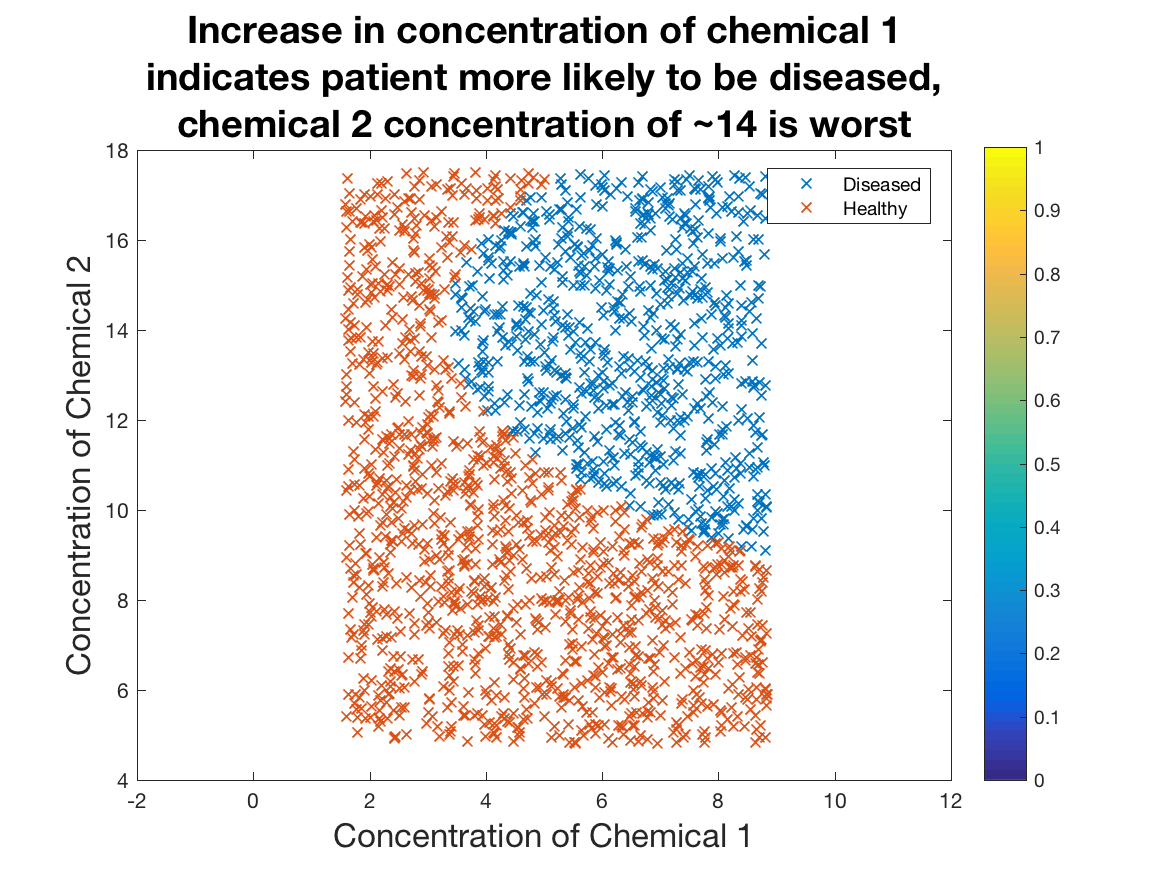
\includegraphics[width=\textwidth]{MLnewData.png}
		\caption{Maximum Likelihood classification of new data}
		\label{fig:model0}
	\end{subfigure}
	\begin{subfigure}[b]{.49\textwidth}
		\includegraphics[width=\textwidth]{MLWONnewData.png}
		\caption{Maximum Likelihood WON classification of new data}
		\label{fig:model1}
	\end{subfigure}
	\begin{subfigure}[b]{.49\textwidth}
		\includegraphics[width=\textwidth]{MAPnewData.png}
		\caption{Maximum a posteriori classification of new data}
		\label{fig:model2}
	\end{subfigure}
	\begin{subfigure}[b]{.49\textwidth}
		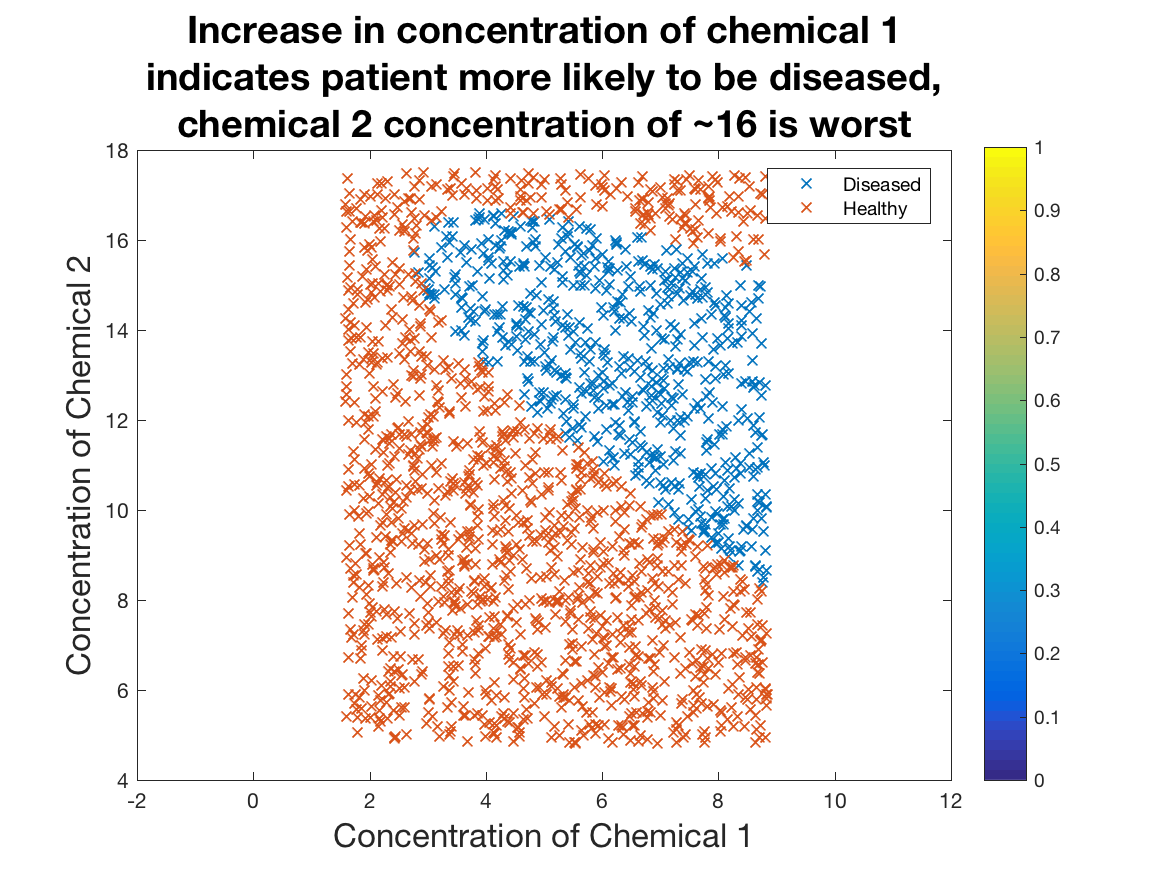
\includegraphics[width=\textwidth]{MAPWONnewData.png}
		\caption{Maximum a posteriori WON classification of new data}
		\label{fig:model3}
	\end{subfigure}
	\caption{Comparison of classification of new data by ML, MLWON, MAP, and MAPWON}
	\label{fig:overallC}
\end{figure}

\section{Conclusion}
The Naive assumption has a significant influence on this data set indicating there is a relationship between the attributes. 

ML and MAP had little difference in this case due to limited affect of the prior. The prior had little affect because of the large difference in means and the small covariances.

Considering the hypothesis of the training data - an increase in concentration of chemical 1 and 2 increases the likelihood of a patient being diagnosed as diseased. With the Naive assumption, it almost agrees with our hypothesis. However, we notice that healthy patients appear again above the diseased, therefore, we reject the hypothesis. Without the Naive assumption, there is a negative relationship between the attributes for diseased classification. In other words, if the concentration increases for one chemical but not the other, a patient is more likely diseased. Therefore, we reject the hypothesis for this case also.

\section{Further Comments}
It is safer to classify patients as diseased  and re test for confirmation than classify for healthy when a patient is diseased. In other words, a false negative is more costly than a false positive. This is reinforced by the speed and reduced cost of the urine test. Considering this, it may be better to use the naive assumption to classify. But when diagnosing it would be best to look at both and make an educated decision.

We also discover the rate at which the ML (or MAP) decreases for diseased patients compared to healthy. Looking at Figures \ref{fig:cml1} and \ref{fig:cml3}, we see this by the close proximity of contours for the diseased compared to the healthy. This means, for an increase in chemical concentration, there is a point where the likelihood of being diseased becomes less than being healthy. This can be explained by imaging two lines with different slopes and y intercepts, where the y value is the likelihood of the class and slope represents the proximity of contour lines. If we imagine line 1 has a larger y intercept (larger initial likelihood) but greater negative slope (closer contour lines) than line 2, then there is a point where y value of line 1 becomes less than line 2 due to the greater negative slope. This point is when line 2 has greater y value  i.e. when there is greater likelihood of class 2.

The probability contours in Figures \ref{fig:CMLprob} and \ref{fig:CMAPprob} reinforce what we deduced in the density contour plots. This is because they are very much dependent on each other. To generate the probability contours we normalise the maximum likelihood by dividing it with the sum of the ML (or MAP) for each class. Therefore, the probability contour plots are the normalised versions of the maximum likelihood density plots. These are useful as the contours represent actual probabilities and also indicate the decision boundary for the 2 classes.









